\chapter{Background}
\label{chap:background}
% Explain what this chapter is all about!
In this chapter we will give an introduction to background for our master thesis as well as the tools, technology and previous research that made it all possible. 

    \section{EiT VR Village}
        \subsection{What is EiT?}
        Experts in Teamwork(EiT) is a compulsory subject for Master students at NTNU. There are about 80 villages, each with its unique village theme. The general theme for the villages are problem areas from society and working life. In each village, students are divided into groups and are to define their own project related to the village theme.\cite{EiTAbout}
        
        The point of EiT is for students to develop interdisciplinary teamwork skills. By composing each EiT village of students from a wide range of disciplines, each student will learn how to work together in interdisciplinary groups. There is also a focus on reflection of one's own contribution in a team, and reflection on the team altogether.\cite{EiTAbout}
    
        \subsection{VR/AR for learning and training}
        This thesis has a strong connection to the EiT village "Virtual and Augmented Reality for Learning and Training". This village already had most of the required resources in place for the students to use, and the course description and goal of the village aligns with our motivation for exploring the possibilities in this field.
        
        On NTNU's page about the village (Translated to English): \emph{"Virtual and augmented reality (VR/AR) have had an explosive development the last years. This opens up big opportunities in an educational context. For example, safely and easily experience highly realistic educational situations that is not easily accessible in real life, like exploring the seafloor, burning buildings, or war zones. With this technology the students get access to visualizations and simulations that can contribute to a better understanding of syllabus and to better acquiring of skills, e.g. in a virtual lab or operation room.}
        
        \emph{Virtual reality also opens up new opportunities for remote education were students can work together in a virtual hospital or cooperate with students at NTNU Gjøvik and Ålesund. There are being developed games like Pokemon GO to give an introduction to local history. VR/AR can be used in adult education for everything from emergency response training and training of neurosurgeons to work training under direction from NAV. Virtual reality is also used for therapy and medical treatment, e.g. for mental and physical training and stimuli, for disabled people and the elderly."} \cite{EiTVRLandsby}
        
    \section{NTNU Dragvoll VR Lab}

    \section{Concepts}
    
        \subsection{Virtuality Continuum}
        The Virtuality Continuum(VC), as shown in Figure \ref{fig:virtualcontinuum}. \emph{"Is a concept which relates the mixture of classes of objects presented in any particular display situation."}\cite{Milgram1994} This article, "\emph{A Taxonomy of Mixed Reality Visual Displays}" by Paul Milgram and Fumio Kishino\cite{Milgram1994} introduces the concept of a "virtuality continuum" to describe the range of environments shown on any particular display. The articles focus on the taxonomy of Mixed Reality displays, and is also one of the earliest adapters of the concept of Mixed Reality.
        \begin{figure}[!ht]
            \centering
            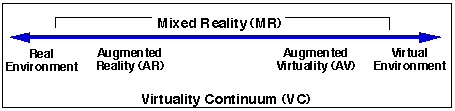
\includegraphics[scale=1]{figures/virtualcontinuum.png}
            \caption{Simplified representation of a "virtuality continuum".\cite{Milgram1994}}
            \label{fig:virtualcontinuum}
        \end{figure}
        
        \subsubsection{Virtual Reality}
        Using Milgram's and Kishinos's description of Virtual Reality(VR) from their paper.\cite{Milgram1994} VR is the concept of a virtual space where the user is fully immersed in a virtual world, usually through a Head Mounted Display(HMD). This means that the environment, and everything the user sees and interacts with is completely synthetic. The environment can emulate the real world and seem like reality, be it fiction or otherwise; or this virtual environment might be a world where our physical laws do not apply. On the virtuality continuum, as shown in Figure \ref{fig:virtualcontinuum}, this type of environment resides on the furthest extreme, opposite the real environment.
    
        \subsubsection{Augmented Reality}
        Augmented Reality(AR) is the concept of a real environment with digital elements superimposed, enhancing the users perception of reality.This is achieved by rendering these digital "\emph{holograms}" on a transparent display which the user sees through(e.g. Microsoft's Hololens or Magic Leap. The same effect can also be achieved by superimposing the digital elements onto video captured by a camera in real-time.
        
        \subsubsection{Mixed Reality}
        As shown in Figure \ref{fig:virtualcontinuum}, a Mixed Reality(MR) display can reside anywhere between the extremes of the virtuality continuum\cite{Milgram1994}. The technology has moved on since 1994, when the paper by Kishino and Milgram was published. \emph{"Since then, the application of mixed reality goes beyond displays but also includes environmental input, spatial sound, and location."}\cite{wdc-mr}
        
        Microsoft, especially, has expanded on the application of Mixed Reality. And in the article "What is mixed reality?"\cite{wdc-mr}. MR is described like this: \emph{"Most mobile phones on the market today have little to no environmental understanding capabilities. Thus the experiences they offer cannot mix between physical and digital realities. The experiences that overlay graphics on video streams of the physical world are augmented reality, and the experiences that occlude your view to present a digital experience are virtual reality. As you can see, the experiences enabled between these two extremes is mixed reality"}\cite{wdc-mr}. This spectrum is found in Figure \ref{fig:mrspectrum}
        
        \begin{figure}[!ht]
            \centering
            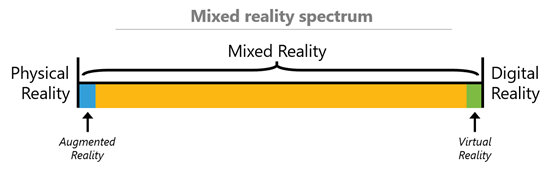
\includegraphics[scale=1]{figures/mixedrealityspectrum.png}
            \caption{The Mixed Reality Spectrum\cite{wdc-mr}}
            \label{fig:mrspectrum}
        \end{figure}
        
        In Figure \ref{fig:mrdevicetypes} the two main device types that deliver Windows Mixed Reality is listed. These are: Holographic devices, which has the ability to place digital content in the real world;\cite{wdc-mr} and Immersive devices, which has the ability to hide the physical world and replace it with a digital experience.\cite{wdc-mr} 
        \begin{figure}[!ht]
            \centering
            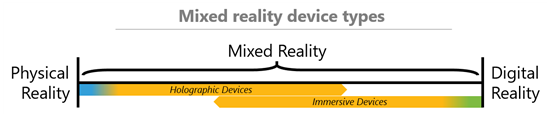
\includegraphics[scale=1]{figures/mixedrealityspectrumdevicetypes.png}
            \caption{Mixed reality device types.\cite{wdc-mr}}
            \label{fig:mrdevicetypes}
        \end{figure}
        
        \subsection{Holograms}
        
        \subsection{Immersion} % Research and definition of what immersion means in the context of VR
        Immersion in relation to computer games is "used to describe the degree of involvement with a game" \cite{Brown2004}. In the paper by Brown in 2014 he defines three different levels of immersion: Engagement, engrossment and total immersion. Each level has its own barriers that needs to be removed for that level of immersion to be possible. Entering a higher level of immersion is correlated with having a higher level of concentration and focus \cite{Jennett2008}. For IVR-Connection this is one of the concepts that can give the user an advantage over collaborating in "real life".
        
        \subsection{Presence} % Research and definition of what presence means in the context of VR
        Jennet et al. presents two different perspectives on the definition of presence \cite{Jennett2008}. The first has basis in the rationalistic tradition, and defines presence as a psychological sense of being in a virtual environment \cite{Slater1994}. With this perspective the level of presence has to be evaluated through user feedback. The other bases itself on the Heideggerian/Gibsonian metaphysics, and relates presence to the ability of "successfully supported action in the environment" \cite{Zahorik1998}. With this perspective presence can be evaluated through empirical means. Presence and immersion have a lot in common and are often used interchangeably. However, Jennet et al. argues that presence is a state of mind, while immersion is an experience in time \cite{Jennett2008}. With this distinction presence and immersion are allowed to overlap, but it is also possible to have one without the other.
        
        \todo{Explain "Ready-In-Hand" and "throwness". This relates to what presence means for mixed reality}
    
    \section{Technology}
    % What technology are we using.
    In this section we will cover the technology that made everything possible. This master is based on cutting edge technology from Microsoft and Unity.
    
        \subsection{Universal Windows Platform}
        % About UWP. What is it and why we use it
        Universal Windows Platform (UWP) provides a common app platform for every device that runs Windows 10. An UWP app is written in C++ /WinRT or C++ /CX and has access to the Win32 APIs that are part of the UWP. These Win32 APIs are implemented by all Windows 10 devices.\cite{wdc-UWP} Examples of devices running Windows 10 are: Desktop computers, phones, XBOX and Hololens.
        
        \subsection{Mixed Reality Toolkit}
        % What is it and why we use it
        \emph{"The Mixed Reality Toolkit is a collection of scripts and components intended to accelerate development of applications targeting Microsoft HoloLens and Windows Mixed Reality headsets. The project is aimed at reducing barriers to entry to create mixed reality applications and contribute back to the community as we all grow."}\cite{MRToolkitReadme}
    
        \subsection{Unity}
        % What is it and why we use it
        Unity is a game engine for creating 2D, 3D, VR, AR and MR games and apps. It has its own graphics engine and a full-featured editor that enables you to create games, and deliver your content to virtually any media or device. Unity also features services like cloud building, multiplayer network, version control and analytics. Unity is also at the forefront of the growing VR market. An estimated 90\% of Samsung Gear VR games and 53\% of Oculus Rift (games at launch) were[sic] Made With Unity. \cite{UnityAbout}
        
        \subsection{Unreal}
        One of the oldest and most used game engines (20 years). Been used by multiple award winning AAA games. Written in C++ and is highly optimized for PC, VR and Mobile platforms.
        Visual coding in C++ using blueprints.
    
        \subsection{Hololens}
        The Hololens is Microsoft's holographic device. Using inside-out tracking, it is a fully mobile head mounted device running Windows 10. It has full six-degrees of freedom movement and uses a see-through display to render the "\emph{holograms}".
    
        \subsection{Immersive Headsets}
        Under the Mixed Reality Moniker, the Immersive Headsets are VR headsets that uses built-in inside-out tracking. With no need for external sensors, and only one cable for connection with the PC; One can enjoy VR from anywhere. Headsets are provided by multiple different big name retailers, all providing their own designs and solutions for the platform.
    
    \section{Related Work}
        
        \subsection{IVR-Connection}
        % About this program and how it fits in with the vision and idea from 4C1R
        Program made by Nicklas to test cooperation in VR.
        
        \subsection{Virtual Reality Spectating}
        
        \subsection{Medical Procedural Training in Virtual Reality}
